\documentclass[11pt,a4paper]{ltjsarticle}
% Compile with LuaLaTeX

% =========================
% Packages
% =========================
\usepackage{luatexja}
\usepackage{graphicx}
\usepackage{hyperref}
\usepackage{amsmath,amssymb,mathtools}
\usepackage{xcolor}
\usepackage{float}
\usepackage{subcaption}
\usepackage{booktabs}
\usepackage{enumitem}
\usepackage{geometry}

\geometry{margin=22mm}
\setcounter{tocdepth}{3}
\setlength{\parskip}{0.6mm}

% =========================
% User information
% =========================
\title{Weekly Report: Ultra-High-Pressure ODMR --- \\ Why should the anvil culet be [111]? Testing the $E=0$ argument}
\author{Risei Abe}
\date{Week: 2026/08/02 -- 2026/08/08}

% =========================
% Custom commands
% =========================
\newcommand{\sectionblock}[1]{%
  \vspace{2mm}
  {\large\textbf{#1}}
  \vspace{1mm}

}

\newcommand{\todo}[1]{\textcolor{red}{#1}}

\begin{document}

\maketitle

% =========================================================
% 1. Question / Purpose
% =========================================================
\sectionblock{Question}

\begin{quote}
A [111] culet puts one NV family exactly along the load axis, so that family keeps its $C_{3v}$ symmetry and its transverse-strain splitting $E$ vanishes; does that argument actually make [111] the better choice for ODMR sensitivity at 120\,GPa, compared with a [100] culet where all four families are equivalent?
\end{quote}

% =========================================================
% 2. Hypothesis
% =========================================================
\sectionblock{Hypothesis}

If the axial family on a [111] culet has $E=0$ and therefore no transverse-strain broadening, it should give the narrowest line and win despite carrying only $1/4$ of the NV population, whereas [100] keeps all four families but pays a linewidth penalty $\propto |dE/dt|\,\delta t$ from the spread $\delta t$ in deviatoric stress across the culet.

% =========================================================
% 3. Evidence / Interpretation
% =========================================================
\sectionblock{Evidence / Interpretation}

\begin{figure}[H]
  \centering
  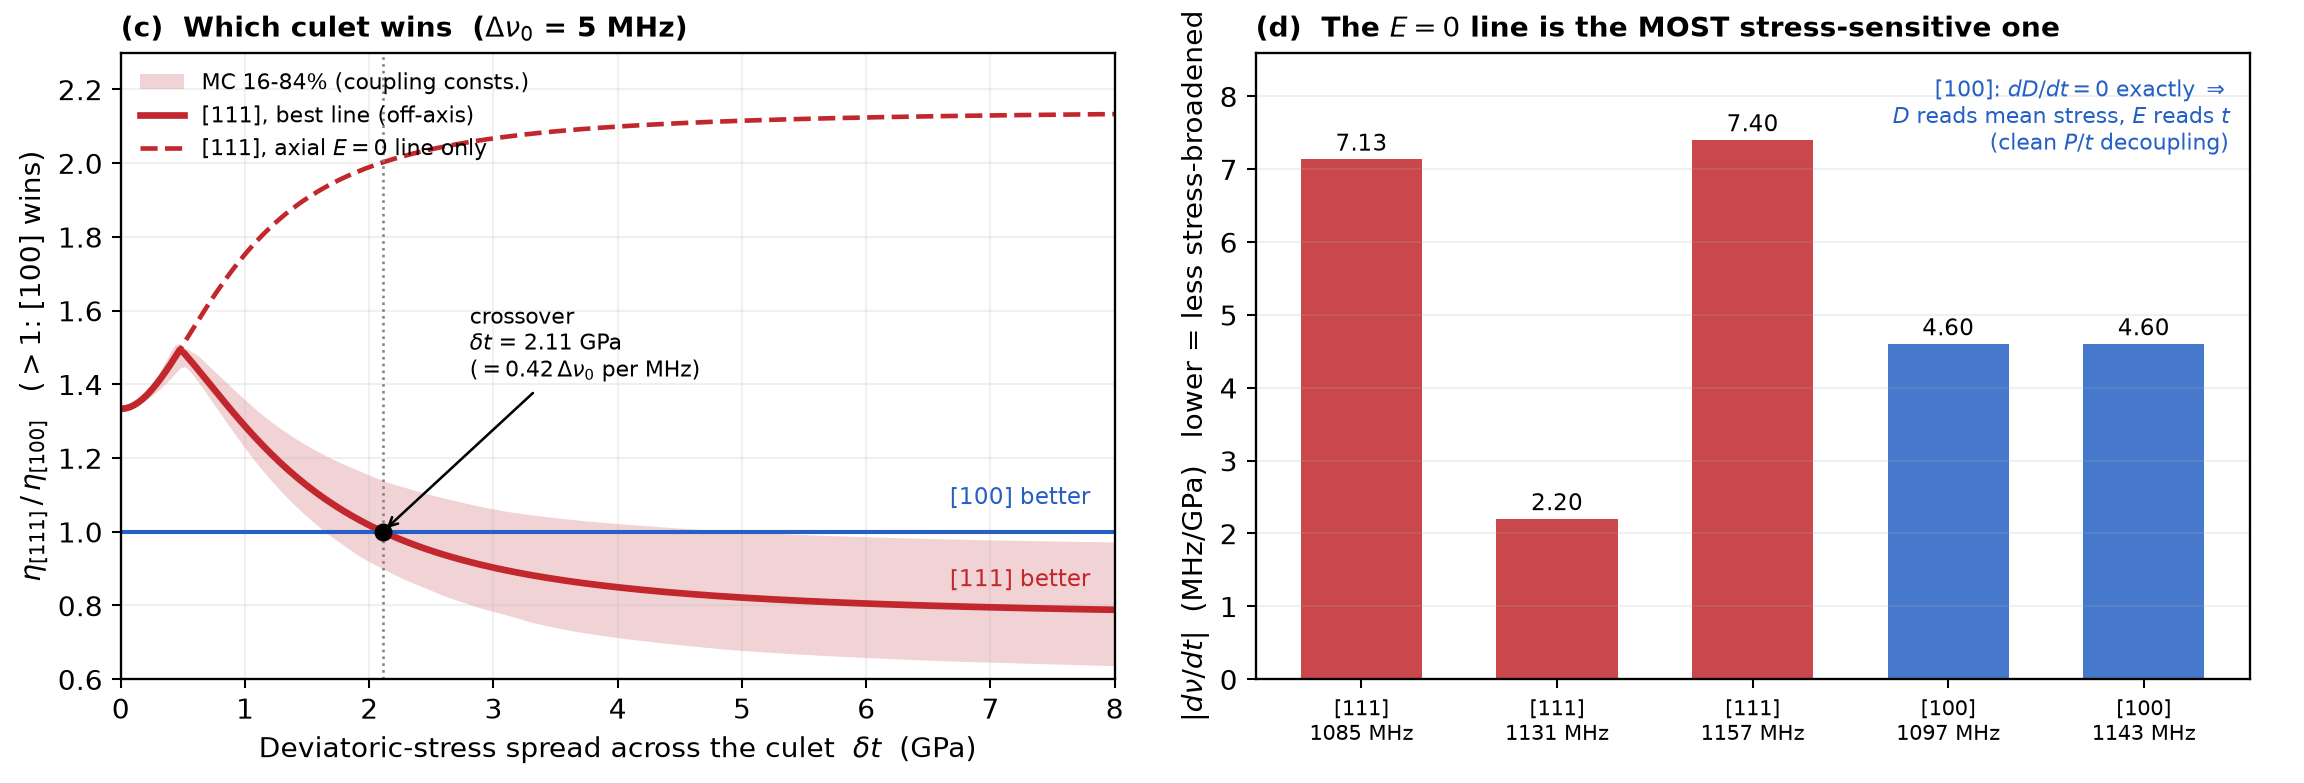
\includegraphics[width=0.99\linewidth]{image/anvil_culet_decision.png}
  \vspace{-1mm}
  \caption{Left: $\eta_{[111]}/\eta_{[100]}$ vs.\ the deviatoric-stress spread $\delta t$, for the best [111] line and for the axial $E=0$ line alone, with a Monte-Carlo band over the Barson spin-stress constants. Right: $|d\nu/dt|$ of every line; the $E=0$ line is the steepest one.}
  \label{fig:culet}
\end{figure}
\vspace{-3mm}

\begin{itemize}[leftmargin=8mm]
  \item The symmetry argument itself holds exactly ($E=0$ and $dE/dt=0$ for the axial family), but that line is nevertheless the \emph{most} deviatoric-stress-sensitive one in the problem, $|dD/dt| = |2a_2| = 7.40$\,MHz/GPa versus 4.60\,MHz/GPa for [100], and with only 0.375 of the PL dipping it loses to [100] by $1.33\times$ to $2.14\times$ at every $\delta t$.
  \item {[111]} does win, but above $\delta t \approx 0.42\,\Delta\nu_0$ (GPa per MHz of intrinsic width, i.e.\ 2.1\,GPa for $\Delta\nu_0 = 5$\,MHz) and through the \emph{off-axis} families, whose line at $|d\nu/dt| = 2.20$\,MHz/GPa is the narrowest available --- so the correct reason to pick [111] is the opposite of the usual one.
\end{itemize}

% =========================================================
% 4.  Gap / Failure
% =========================================================
\sectionblock{Gap / Failure}

\begin{itemize}[leftmargin=8mm]
  \item The model scores only $\eta \propto \Delta\nu/(C\sqrt{R})$ at zero bias field, so it cannot see the genuine [111] advantage for vector magnetometry, where a field along the axial NV is unmixed by $E$.
  \item It also says nothing about the dominant real-world reason for [111] anvils --- the higher compressive strength and the cleavage-plane geometry that decide whether the anvil survives 120\,GPa at all.
\end{itemize}

% =========================================================
% 5. Next Step
% =========================================================
\sectionblock{Next Step}

Fold the $\delta t$-dependent linewidths from this model into the background-aware sensitivity code so that the culet choice, the excitation wavelength and the background level are optimised together rather than one at a time.

% =========================================================
% 9. References
% =========================================================
\sectionblock{References}

\begin{enumerate}[leftmargin=8mm]
  \item M.\,S.\,J.\ Barson \emph{et al.}, ``Nanomechanical Sensing Using Spins in Diamond,'' Nano Lett.\ \textbf{17}, 1496 (2017) --- spin-stress constants $a_1, a_2, b, c$.
  \item P.\ Udvarhelyi \emph{et al.}, Phys.\ Rev.\ B \textbf{98}, 075201 (2018) --- spin-strain Hamiltonian conventions.
  \item M.\,W.\ Doherty \emph{et al.}, Phys.\ Rev.\ Lett.\ \textbf{112}, 047601 (2014) --- NV under pressure.
  \item Repository: \texttt{code/anvil\_orientation.py}, \texttt{code/fig6\_anvil\_orientation.py} (this analysis).
\end{enumerate}

\end{document}
